
%%%%%%%%%%%%%%%%%%%%%%%%%%%%%%%%%%%%%%%%%%%%%%%%%%%%%%%%%
%%%% BALLISTIC OBJECT %%%%%%%%%%%%%%%%%%%%%%%%%%%%%%%%%%%
%%%%%%%%%%%%%%%%%%%%%%%%%%%%%%%%%%%%%%%%%%%%%%%%%%%%%%%%%

\subsection{Endoathmospheric flight of a ballistic projectile}\label{sec:ballistic}
Let us consider a situation where a ballistic projectile is launched
from the ground into the air. We assume that the situation is governed by Newtonian
mechanics and that the projectile experiences a constant known gravitational
force, directed towards the ground. In addition we assume a \emph{constant}
drag force directed orthogonally to the gravitational force. This is clearly
an oversimplification, since in a more realistic model the drag
force should be proportional to velocity and directed against it. Furthermore
the drag force is highly dependent on air density and so on the altitude \parencite{ristic2004beyond}.
Nevertheless, we make the aforementioned simplification to keep to resulting
SSM linear. The modeling error is mitigated slightly by introducing
additive white noise to both forces.

We obtain a sequence of range measurements with a radar,
so that our data consists of the noisy two dimensional locations 
of the object as measured at time points $\brac{t_k}_{k=1}^T$.
We assume a constant interval $\tau$ between the time points. With these 
considerations, the system can be cast into a linear-Gaussian SSM. 

In continous time and for a single coordinate $\chi$, 
the dynamics can now be written as
\begin{align}
	\dod{}{t}\bm{\chi(t) \\ \dot{\chi}(t) } &= 
	\bm{0 & 1\\0 & 0}\bm{\chi(t) \\ \dot{\chi}(t) } + \bm{0\\1}g_\chi + \bm{0\\1}\beta(t),
	\label{eq:ct_linear}
\end{align}
where $g_\chi<0$ is the mean of the force and $\beta(t)$ can be considered
a white noise process with variance (or spectral density) $\sigma^2_\chi$. 
Thus the state contains the position and its first time derivative, the velocity. 

% with
% \begin{align}
% 	\x(t) &= \bm{x(t) & \dot{x}(t) & \ddot{x}(t) & y(t) & \dot{y}(t) & \ddot{y}(t)}^\tr\\
% 	\v{F}&=\bm{
% 	&&1&&&\\
% 	&&&1&&\\
% 	&&&&1&\\
% 	&&&&&1\\
% 	&&&&&\\
% 	&&&&&\\
% 	}
% 	\label{tablelabel}
% \end{align}

To discretize the dynamics, we will apply a simple integration scheme where 
$\x(t)=\x(t_k)$ when $t\in\big[t_k,t_{k+1}\big)$ \parencite{bar2004estimation}.
The system will be modeled in two dimensional Cartesian coordinates with
two state components for position and two for velocity, giving $d_x=4$. The state at time $k$ is then
\begin{align}
	\xk &=
	\bm{\chi_k & \dot{\chi}_k  
	  & \gamma_k & \dot{\gamma}_k }^\tr
	\label{eq:ballistic2D_state}
\end{align}
where $\dot{\chi}_k = \eval{\dod{\chi(t)}{t}}_{t=t_k}$ and analogously for $\dot{\gamma}_k$.
The corresponding measurement is given by
\begin{align}
	\yk &= \bm{\chi_k & \gamma_k }^\tr + \v{r}_k,
	\label{eq:ballistic2D_measurementsl}
\end{align}
where $\v{r}_k$ is a white noise process with variance $\sigma^2_r$.
%
The discrete time linear-Gaussian SSM can now be written as
\begin{align}
	\begin{aligned}
	\x_k &= \v{A}\xkk+\v{u}+\q_{k-1},\qquad & 
	\q_{k-1} &\sim \N{\v{0}}{\v{Q}},\\
	\yk &= \v{H}\xk+\v{r}_k, & 					
	\v{r}_k 	&\sim \N{\v{0}}{\sigma_r^2\v{I}},
	\end{aligned}\label{eq:ballistic_model}
\end{align}
where
\begin{align*}
	\v{A}&=\bm{
	1& \tau & 	& 		\\
	 &	1	& 	&		\\
	 &		& 1	& \tau 	\\
	 &		&	& 1
	},
	&
	\v{u} &= \bm{0 \\ g_\chi \\ 0 \\ g_\gamma},\\
	%
	\v{Q}&=\bm{
	\sfrac{1}{3}\sigma_\chi^2\tau^3 & \sfrac{1}{2}\sigma_\chi^2\tau^2 & 	& 		\\
	\sfrac{1}{2}\sigma_\chi^2\tau^2 &	\sigma_\chi^2\tau & 	&		\\
	 &		& \sfrac{1}{3}\sigma_\gamma^2\tau^3	& \sfrac{1}{2}\sigma_\gamma^2\tau^2 	\\
	 &		&	\sfrac{1}{2}\sigma_\gamma^2\tau^2 & \sigma_\gamma^2\tau
	},
	&
	\v{H} &= \bm{1 & 0 & 0 & 0 \\ 0 & 0 & 1 & 0}.
\end{align*}
Additionally, the initial state $\x_0$ is assumed to be known
with $\x_0=\bm{0 & \cos(\alpha_0)v_0 & 0 & \sin(\alpha_0)v_0}^\tr$.

Figure~\ref{fig:ballistic2D_simulation} presents an example trajectory with
the hidden state components obtained by simulation and the corresponding
simulated noisy measurements. The simulated model was the
linear-Gaussian SSM in Equation~\eqref{eq:ballistic_model} with  
the parameter values presented in Table~\ref{table:ballistic_param}.

\begin{table}[htbp]
\caption{Parameter values used for simulation in Section~\ref{sec:ballistic}}
\label{table:ballistic_param}
\centering
\footnotesize
\begin{tabular}{>{$}c<{$}Ss@{\hspace{1.5cm}}>{$}c<{$}Ss}
\toprule
\multicolumn{1}{c}{Parameter}&%
\multicolumn{1}{c}{Value}&%
\multicolumn{1}{c@{\hspace{1.5cm}}}{Unit}&%
\multicolumn{1}{c}{Parameter}&%
\multicolumn{1}{c}{Value}&%
\multicolumn{1}{c}{Unit}\\
\midrule
	\sigma_\chi		&	1.2			&	m			&	\tau			&	0.01 		& s\\
	\sigma_\gamma 	&	0.8			&	m			&	\sigma_r		& 	2.5 		& m	\\	 	
 	g_\chi			&	-1.8		&	m/s^2		&	\alpha_0		& 	60 		& \degree\\	 	
	g_\gamma 		&	-9.81		&	m/s^2		&	v_0 			&	40	 	& m/s\\
\bottomrule	 	
\end{tabular}
\end{table}

Let us then proceed to estimating some of the parameters by using the noisy
measurements as input to the two parameter estimation methods we have been considering.
We choose parameters $\Th_{\mathrm{B}}=\brac{g_\chi,g_\gamma,\sigma_r}$, which are the
accelerations caused by the drag force and gravitation as well as the measurement noise
standard deviation. The true values, that is, the values which were used for generating the
measurements are presented in Table~\ref{table:ballistic_param}. To inspect the effect of
the initial guess as well as well as that of the specific measurement dataset, we ran
$M=100$ simulations with the initial estimate for each parameter $\theta_i$ picked 
from the uniform distribution $U\brak{0,2\theta_i^*}$, where $\theta_i^*$ is the true generative value
for parameter $i$ given in Table~\ref{table:ballistic_param}. The lengths of
the simulated measurent datasets were around $N\approx 1400$ with some variance caused by always stopping
the simulation when $\gamma_k<0$ for some $k$. For each simulated dataset and the associated
initial estimate we ran the EM and the BFGS parameter estimation methods for joint estimation
of the three parameters. 

In this case one can find closed form expressions for all three parameters in the EM M-step.
The M-step equations for linear-Gaussian SSMs, presented in Equations \eqref{eq:EM_M_A}, 
\eqref{eq:EM_M_H}, \eqref{eq:EM_M_Q} and \eqref{eq:EM_M_R}, do not include one
for estimating the constant input $\v{u}$, which in this case contains the accelerations. It is not
difficult to derive however and for this particular model it reads
\begin{align}
	\v{u}_{j+1} =&\, \frac{1}{2T\tau^2}\bm{0&1&0&0\\0&0&0&1}\nonumber\\
	&\times\fparen[\Big]{3\fparen[\big]{m_{0|T}-m_{T|T}}+
	\tau\fparen[\big]{2\sum_{k=1}^Tm_{k|T}+\sum_{k=1}^Tm_{k-1|T}}}
	\label{eq:EM_M_u}.
\end{align}

The BFGS implementation used was the \texttt{fminunc} function included
in the \matlab{} Optimization Toolbox \parencite{fminunc}. It is intended
for general unconstrained nonlinear optimization and implements other
methods in addition to BFGS. To force BFGS, \texttt{fminunc} should be called
in the following way
\begin{lstlisting}[language=Matlab]
opt = optimset(@fminunc);
opt.GradObj = 'on';
opt.LargeScale = 'off'; % use BFGS
% lhg = objective function and gradient 
% [lh(x),lh'(x)] = lhg(x)
% p0 = initial estimate
p_min = fminunc(@lhg,p0,opt);
\end{lstlisting}

The likelihood convergence for both methods is presented in Figure~\ref{fig:ballistic_lh}.
It is important to note that the iteration numbers are
not directly comparable between the parameter estimation methods so that one
shoudn't attempt to draw conclusions on the \emph{relative} convergence rate betweeen the methods
based on the convergence plots. \todo{explain the computational complexity differences}
\todo{Present the average learning curves with normalized iterations?}

The parameter convergence results are presented in Figure~\ref{fig:ballistic_est},
which contains eight separate panels: one per parameter and estimation method and
the likelihoods for both estimation methods. One line is plotted
in every panel for every simulated dataset and the panels display their quantities
as a function of the iteration number of the estimation method. The convergence
profiles show a lot of variability between the methods and between the parameters but
the means of the converged estimates seem to agree very well with the generative values
in all cases. Also $g_\gamma$ and $\sigma_r$ show very little variance in the
converged estimate compared to $g_\chi$. In any case, according to the asymptotic
theory of the ML/MAP estimates, the variance should go to zero as the amount of data
approaches infinity.

Finally, Table~\ref{table:ballistic_restults} presents the averaged final
results. Both methods seem to obtain the same results and in fact they agree to the first six decimal places. 
This is to be expected, since as mentioned earlier, they can be proved to compute the same quantities 
in the linear-Gaussian case. The fact that
the results differ after the sixth decimal place can be explained by differing
numerical properties of the two algorithms. In case of $g_\gamma$ and $\sigma_r$,
the estimates agree exactly at least to three decimal places with the generative
values, whereas $g_\chi$ is correct up to two decimal places. Since we are using
unbiased estimates, the estimation error could be diminished up to the order of the machine
epsilon by simulating more data points \todo{Is this true or does it depend on the numerical properties?}.
As a conclusion, it seems that in this case the estimation problem was too simple to bring
about noticeable differences in the performance of the parameter estimation methods.

\begin{figure}[htbp]%
    \centering%
    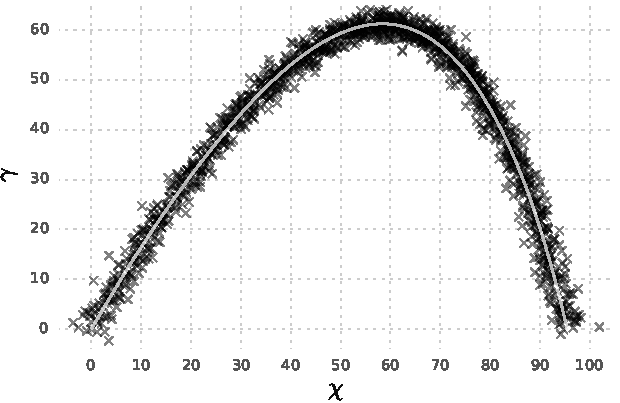
\includegraphics{img/ballistic_trajectory}%
	\caption{A simulated trajectory (white line) and noisy
	measurements (black crosses) from 
	the linear-Gaussian SSM \eqref{eq:ballistic_model}. 
   	The coordinates are in meters.
   	The projectile is simulated for approximately $7$
   	seconds and there are $T=1396$ measurements.
   	}\label{fig:ballistic2D_simulation}
 \end{figure}

\begin{figure}[htbp]%
    \centering%
	\makebox[\textwidth]{%
    \begin{subfigure}[t]{0.5\textwidth+0.4in}%
    	\caption{EM}\label{fig:ballistic_lh_em}%
    	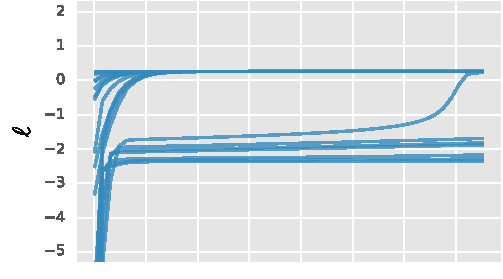
\includegraphics{img/ballistic_lh_em}%
    \end{subfigure}%
    \begin{subfigure}[t]{0.5\textwidth+0.4in}%
		\caption{BFGS}\label{fig:ballistic_lh_bf}%
		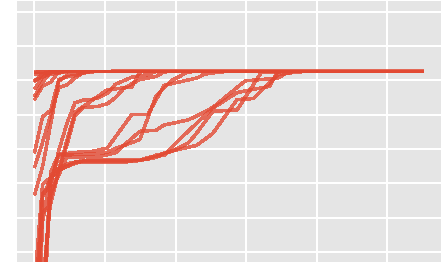
\includegraphics{img/ballistic_lh_bf}%
    \end{subfigure}}
    \caption{Convergence of the likelihood for $M=100$ simulated datasets
    with varying initial parameter estimates. 
    Both EM in \subref{fig:ballistic_lh_em} and BFGS
    in \subref{fig:ballistic_lh_bf} converge to the same
    likelihood value.}\label{fig:ballistic_lh}
\end{figure}
    

%\parencite{ristic2004beyond,Ratna2008,Lindsten2010}
 
 \begin{figure}[htbp]%
    \centering%
    \makebox[\textwidth]{%
    \begin{subfigure}[t]{0.5\textwidth+0.4in}%
    	\caption{EM}
    	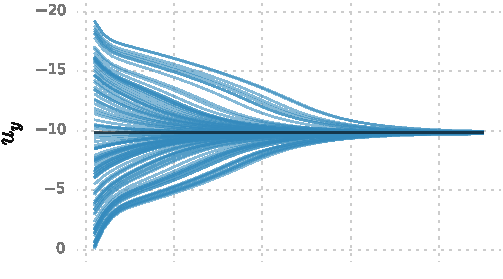
\includegraphics{img/ballistic_em_uy}%
    \end{subfigure}%
    \begin{subfigure}[t]{0.5\textwidth+0.4in}%
		\caption{BFGS}
		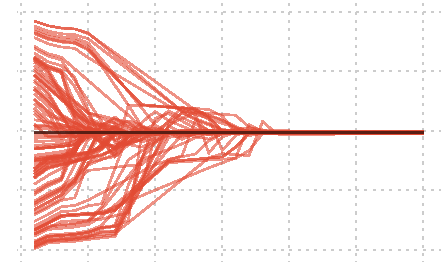
\includegraphics{img/ballistic_bf_uy}%
    \end{subfigure}}\\%
    \makebox[\textwidth]{%
    \begin{subfigure}[t]{0.5\textwidth+0.4in}%
    	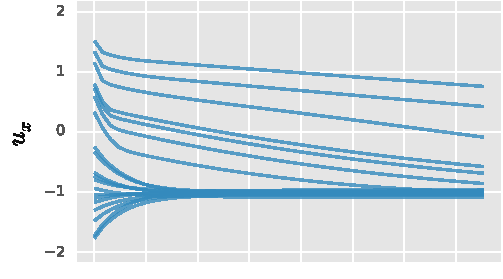
\includegraphics{img/ballistic_em_ux}%
    \end{subfigure}%
    \begin{subfigure}[t]{0.5\textwidth+0.4in}%
		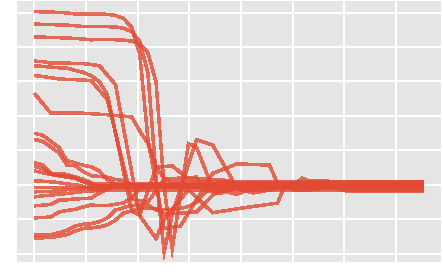
\includegraphics{img/ballistic_bf_ux}%
    \end{subfigure}}\\%
    \makebox[\textwidth]{%
	\begin{subfigure}[b]{0.5\textwidth+0.4in}%
    	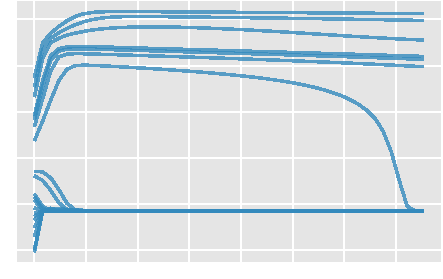
\includegraphics{img/ballistic_em_r}%
    \end{subfigure}%
    \begin{subfigure}[b]{0.5\textwidth+0.4in}%
		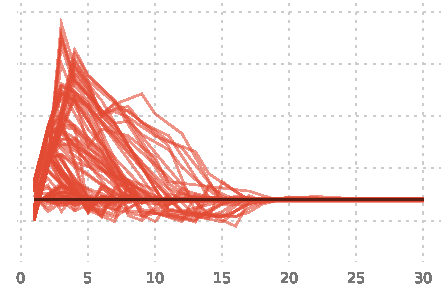
\includegraphics{img/ballistic_bf_r}%
    \end{subfigure}}%
    \caption{Convergence of the parameter estimates with EM and BFGS
    as a function of objective function evaluations in Section~\ref{sec:ballistic}. The black line
    presents the true generative value of the parameter.
    Note that the
    objective functions of the optimization methods differ in their computational complexity, 
    implying that the plots cannot be directly compared in the $x$-axis. }\label{fig:ballistic_est}
 \end{figure}
 
\begin{table}[htbp]
	\caption{Estimated parameter values and the final
	log-likelihood value 
	averaged over $100$ simulations in Section~\ref{sec:ballistic}}
	\label{table:ballistic_restults}
	\centering
	\sisetup{
		table-auto-round,
		table-format = 1.3,
		table-omit-exponent
	}
	\footnotesize
	\begin{tabular}{rSSS}
\toprule
&\multicolumn{1}{c}{{\bfseries $g_\chi$}}&\multicolumn{1}{c}{{\bfseries $g_\gamma$}}&\multicolumn{1}{c}{{\bfseries $\sigma_r$}}\\\otoprule
True&-1.80000&-9.81000&1.50000\\
BFGS&-1.78372&-9.80360&1.49913\\
EM&-1.78372&-9.80473&1.49912\\
\bottomrule\end{tabular}

\end{table} 


\clearpage


%%%%%%%%%%%%%%%%%%%%%%%%%%%%%%%%%%%%%%%%%%%%%%%%%%%%%%%%%%%%%%%%
%%%%%%%%%%%%%%%%%%%% HEART %%%%%%%%%%%%%%%%%%%%%%%%%%%%%%%%%%%%%
%%%%%%%%%%%%%%%%%%%%%%%%%%%%%%%%%%%%%%%%%%%%%%%%%%%%%%%%%%%%%%%%

\subsection{Photoplethysmograph waveform analysis}\label{sec:harmonic}

The second demonstration is concerned with a nonlinear model for
photoplethysmograph (PPG) data, a short sequence of which is presented
in Figure~\ref{fig:ecg_data}. PPG is measured with 
a \emph{pulse oximeter} the functioning of which is based on
emitting light (of which the infrared component is relevant to the PPG)
through for example a finger or an earlobe. Then either the transmitted
or reflected light intensity is measured with a photodiode \parencite{Shelley2007}. 
As to what exactly is the source of PPG is not without controversy,
but as explained by \textcite{Shelley2007}:
%\begin{quotation}
``Conceptually, it is most useful to view the pulse
oximeter waveform as measuring the change in blood
volume (more specifically path length), during a cardiac cycle, 
in the region being studied (typically the fingertip or earlobe)'' (p. 31).
%\end{quotation}
The most important use of the PPG is the calculation of arterial oxygen
saturation, but it can also be used to estimate the heart rate.
In this case a PPG was obtained in connection with a brain imaging study, where
a pulse oximeter was attached to the subject while being analysed with fMRI \parencite{Sarkka2012}.   

A realistic model for this data 
should take into account the quasi-periodic nature of PPG data,
meaning the frequency must be allowed to vary with time.
Following the ideas in \textcite{Sarkka2012}, one possibility
is to write the model as a superposition of noisy resonators
with time-varying frequencies.

In continous time we can write a stochastic differential equation
for the $n$:th harmonic as
\begin{align}
	 \ddot{c}_n(t)&= -\omega(t)^2c_n(t)+\varepsilon_n(t),
	 %\dod[2]{c_n(t)}{t}
	\label{eq:noisy_resonator}
\end{align}
where $c_n(t)$ is the displacement from equilibrium at time $t$.
The angular velocity $\omega$ is related to the frequency $f$
by $\omega(t)=2\pi f(t)$ and  $\varepsilon_n(t)$ is additive
white noise with spectral density $q_n$. For constant frequency and
zero spectral density, the solution of Equation~\eqref{eq:noisy_resonator}
is well known to be $c_n(t)=\exp(i n \omega t+\phi_n)$, where $\phi_n\in\field{C}$ depends on 
the initial conditions.

Writing Equation~\eqref{eq:noisy_resonator} as a vector valued first order differential equation
and dividing the noise and the signal derivative by $n\omega(t)$, we get
\begin{align}
	\dod{}{t}\bm{c_n(t) \\ \widehat{\dot{c}}_n(t)} &= \bm{0 & \omega(t) \\ -\omega(t) & 0}\bm{c_n(t) \\
	\widehat{\dot{c}}_n(t)}+\bm{0\\1}
	\widehat{\varepsilon}_n(t).
	\label{eq:noisy_resonator_vec}
\end{align}
As explained in \textcite{Sarkka2012}, even if Equation~\eqref{eq:noisy_resonator_vec} is not an exact
representation of Equation~\eqref{eq:noisy_resonator}, its discretized version has more appealing
properties than that of the exact version. Furthermore, the process noise can account for some
modeling errors. 

Discretizing Equation~\eqref{eq:noisy_resonator_vec} at equispaced points $\brac{t_k}_{k=1}^T$
with interval $\tau$ and assuming $\omega(t)=\omega(t_k)\equiv \omega_k$ when $t\in[t_k,t_{k+1})$
and that the process noises have equal distributions between the harmonics,
we get the following dynamic model for displacement $x^{(n)}$:
\begin{align}
	\bm{x_k^{(n)} \\ \dot{x}_k^{(n)}} &\sim 
	\N{\bm{\cos(n\omega_k) & \sin(n\omega_k) \\% 
	   -\sin(n\omega_k) & \cos(n\omega_k)}
	   \bm{x_{k-1}^{(n)} \\ \dot{x}_{k-1}^{(n)}}}
	  {\bm{0 & 0 \\ 0 & \tau \sigma^2_x}}.
	\label{eq:dynamic_displacement}
\end{align}
We assume that $\omega_k$ is part of the state and that its dynamics follow 
the previously introduced first order
random walk model:
\begin{align}
	\omega_k \sim \N{\omega_{k-1}}{\tau q_\omega}.
	\label{eq:omega_ar}
\end{align}
The joint dynamic model of $m$ harmonics and $\omega_k$ is then
\begin{align}
	\underbrace{\bm{\omega_k \\ x_k^{(1)} \\ \dot{x}_k^{(1)} \\ \vdots \\  x_k^{(m)} \\ \dot{x}_k^{(m)} }}_{\xk} 
	=
	%\N{
	\underbrace{\bm{1&&&&&\\
		& \cos(\omega_k) & \sin(\omega_k) &&&\\% 
	    &-\sin(\omega_k) & \cos(\omega_k) &&&\\
	    &				  &					& \ddots & &\\
	 &&&& \cos(m\omega_k) & \sin(m\omega_k) \\% 
	 &&&&-\sin(m\omega_k) & \cos(m\omega_k) \\
	}
	\bm{\omega_k \\ x_{k-1}^{(1)} \\ \dot{x}_{k-1}^{(1)} \\ \vdots \\  x_{k-1}^{(m)} \\ \dot{x}_{k-1}^{(m)} }}_{\ffi}
	%}{
	%\v{Q}
	%},
	+ \v{q}_{k-1}
	\label{eq:harmonic_joint}
\end{align}
where
\begin{align}
	\q_{k-1}\sim\N{\v{0}}{
	\underbrace{
		\tau\bm{\sigma^2_\omega&&&&&\\ & 0 &&&& \\ && \sigma^2_x &&& \\ &&& \ddots && \\ &&&& 0 & \\ &&&&& \sigma^2_x}
	}_{\QQ{\Th_{\textrm{P}}}}
	}.
	\label{eq:Q_harmonic}
\end{align}
Our objective is now to find the ML estimate (or, equivalently, the MAP estimate with a uniform prior)
of the parameter $\Th_{\textrm{P}}\equiv \brac{\sigma_\omega,\sigma_x}$ by using both the
gradient based nonlinear optimization approach presented in Section~\ref{sec:grad_nonlinear} and the EM
approach presented in Section~\ref{sec:EM_nonlinear}. We will treat
the rest of the parameters as fixed with the values 
presented in Table~\ref{table:harmonic_param}.
The first component of the parameter, $\sigma_\omega$, is the standard deviation
of the angular velocity and the second, $\sigma_x$, is the standard deviation
of the displacement $x$, shared between the $m=3$ harmonic components. 
It would be quite
difficult to try to estimate these values based only on a priori information, in contrast to $\sigma_r$
which could be obtained from the measurement device (the pulse oximeter).

Since $\QQ{\Th_{\textrm{P}}}$ is diagonal, we can use Equation~\eqref{eq:EM_M_Q}
in the EM M-step and pick the corresponding elements from the resulting full matrix
as our next estimates. Similarly to the analysis of the ballistic projectile in Section~\ref{sec:ballistic}, 
the BFGS implementation used was the \texttt{fminunc} function included in the 
\matlab{} Optimization Toolbox. The CKF filter and CKS smoother of Section~\ref{sec:ckf} were used
as the approximate filtering and smoothing methods respectively. The score function
for BFGS was computed by the recursive sensitivity equations of Section~\ref{sec:grad_nonlinear}.  

To analyze the results' sensitivity to the initial estimate, we ran $M=100$ optimizations
with both methods with the initial estimates drawn from a uniform distribution
on a suitable interval (that the initial estimate was always the
same between the methods). The likelihood convergence for
both methods is presented in Figure~\ref{fig:harmonic_lh}.
We note again that the iteration numbers are
not directly comparable. As can be seen, the EM estimates seem to
converge to values producing identical log likelihood values (on the figure's scale) whereas
the BFGS estimates have at least two modes. In contrast to the linear SSM
analyzed in the previous section, here we can see that the convergence of the EM
is not monotonic in all cases.

The parameter convergence
results are presented in Figure~\ref{fig:harmonic_est},
which contains four separate panels: one per parameter and estimation method. 
One line is plotted in every panel for every optimization run and the panels display their quantities
as a function of the iteration number of the estimation method.
The first thing to note is the vast difference in the behavior of the methods.
The EM estimates are quite predictable and either do not converge at
all (in the case of $\sigma_w$) or converge to the same value (in the case $\sigma_x$).
The BFGS estimates on the other hand seem to have multiple convergent values for both
parameters, depending on the initial estimate.

To get more insight into the behavior of the parameter estimation methods, 
illustration of the converge of $\ell$ as a function of
the logarithms of both $\sigma_\omega$ and $\sigma_x$ is presented
in Figure~\ref{fig:harmonic_3D}. The end points of the runs are marked with black stars.
It seems that there are minor local maximums on either side of the major local maximum
around $\log\sigma_x\approx -3$. Some of the BFGS optimization runs ($31$ out of $100$ to be specific) 
converge to the minor local maximums. However, the BFGS runs that do not converge to the
minor local maximums converge in both paramaters while the EM runs only converge in $\log\sigma_x$.
Since $\ell$ is very insensitive to changes in $\sigma_\omega$ (at least on the range explored),
the variance in the final values for $\sigma_\omega$ for the EM runs has only a negligible
effect in $\ell$.  

Table~\ref{table:harmonic_results} presents 
the averaged final results. We have included two sets of estimates for BFGS:
one set for all $100$ runs and another one averaged over the $69$ runs
that converge to the major local maximum. The standard errors in
BFGS($100$) are relatively enormous as expected. However, the standard errors
of BFGS($69$) are markedly \emph{smaller} across the range when compared to
EM($100$). A probable explanation for this is the the inconvergence of
 $\sigma_\omega$ in EM($100$).



\begin{table}[htbp]
\caption{Parameter values used in the PPG analysis in Section~\ref{sec:harmonic}}
\label{table:harmonic_param}
\centering
\footnotesize
\begin{tabular}{>{$}c<{$}Ss@{\hspace{1.5cm}}>{$}c<{$}Ss}
\toprule
\multicolumn{1}{c}{Parameter}&%
\multicolumn{1}{c}{Value}&%
\multicolumn{1}{c@{\hspace{1.5cm}}}{Unit}&%
\multicolumn{1}{c}{Parameter}&%
\multicolumn{1}{c}{Value}&%
\multicolumn{1}{c}{Unit}\\
\midrule
	m				&	3			&	-			&	\tau			&	0.008 		& s \\
	\sigma_r 		&	0.001			&	V			&&& \\		 	
\bottomrule	 	
\end{tabular}
\end{table}

 
 \begin{figure}[htbp]%
    \centering%
    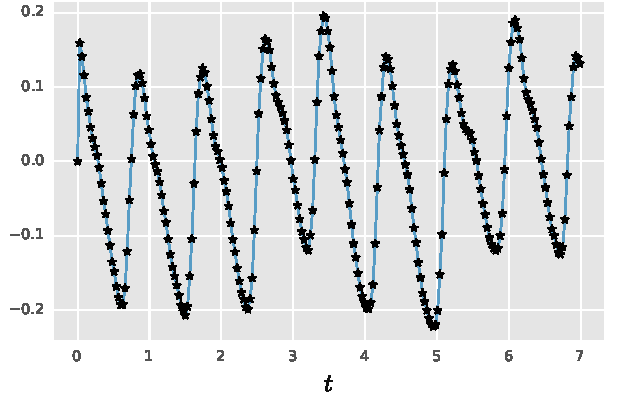
\includegraphics{img/harmonic_trajectory}%
	\caption{%
	A short sequence of the PPG data in Section~\ref{sec:harmonic}. %
   	}
	\label{fig:ecg_data}
 \end{figure}
 
 \begin{figure}[htbp]%
    \centering%
     \makebox[\textwidth]{%
    \begin{subfigure}[t]{0.5\textwidth+0.4in}%
    	\caption{EM}\label{fig:harmonic_lh_em}
    	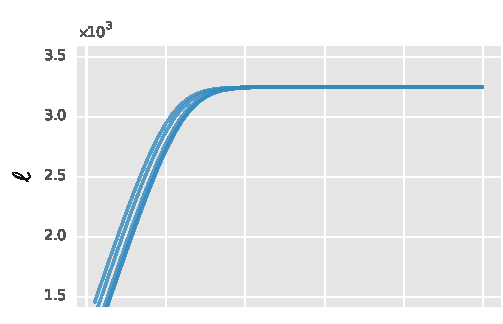
\includegraphics{img/harmonic_em_lh}%
    	%\caption{Convergence of the likelihood with EM}%
		%\label{fig:harmonic_lh_em}%
    \end{subfigure}%
    \begin{subfigure}[t]{0.5\textwidth+0.4in}%
		\caption{BFGS}\label{fig:harmonic_lh_bf}
		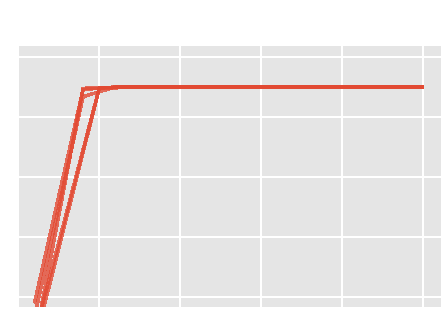
\includegraphics{img/harmonic_bf_lh}%
    \end{subfigure}}%
    \caption{Convergence of the likelihood for $M=100$ simulated datasets
    with varying initial parameter estimates in the photoplethysmograph waveform
    analysis of Section~\ref{sec:harmonic}.% 
    }\label{fig:harmonic_lh}
 \end{figure}
 
 \begin{figure}[htbp]%
    \centering%
    \makebox[\textwidth]{%
    \begin{subfigure}[t]{0.5\textwidth+0.4in}%
    	\caption{EM}\label{fig:harmonic_w_em}
    	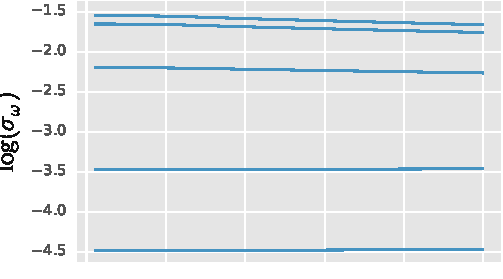
\includegraphics{img/harmonic_em_lqw}%
    \end{subfigure}%
    \begin{subfigure}[t]{0.5\textwidth+0.4in}%
		\caption{BFGS}\label{fig:harmonic_w_bf}
		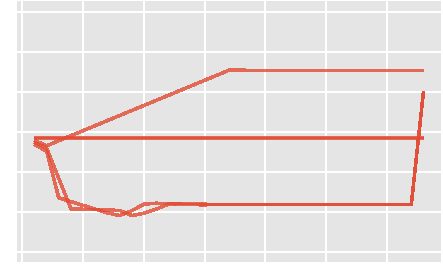
\includegraphics{img/harmonic_bf_lqw}%
    \end{subfigure}}\\%
    \makebox[\textwidth]{%
    \begin{subfigure}[t]{0.5\textwidth+0.4in}%
    	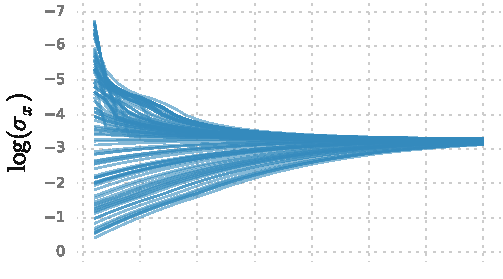
\includegraphics{img/harmonic_em_lqx}%
    \end{subfigure}%
    \begin{subfigure}[t]{0.5\textwidth+0.4in}%
		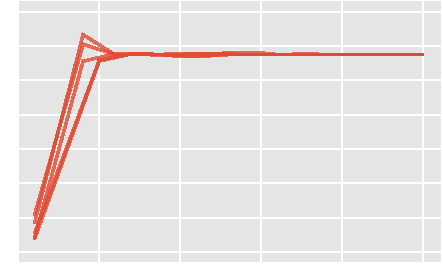
\includegraphics{img/harmonic_bf_lqx}%
    \end{subfigure}}%\\%
    \caption{Convergence of the log-parameter estimates with 
    EM (column \subref{fig:harmonic_w_em}) and 
    BFGS (column \subref{fig:harmonic_w_bf})
    as a function of objective function evaluations in Section~\ref{sec:harmonic}.     
    Note that the objective functions of the optimization methods differ in their computational complexity, 
    implying that the plots cannot be directly compared in the $x$-axis. }
    \label{fig:harmonic_est}
 \end{figure}

\begin{figure}[htbp]%
    \centering%
    \vspace*{-1.5cm}%
    \begin{subfigure}[t]{\textwidth}%
    	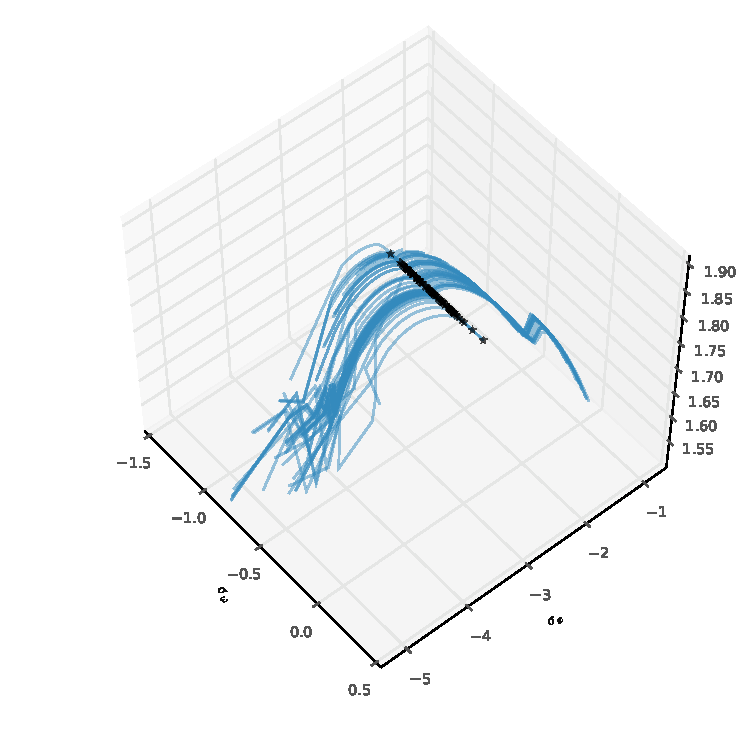
\includegraphics{img/harmonic_3D0}%
    \end{subfigure}\\%
    \vspace*{-1.7cm}%
    \begin{subfigure}[t]{\textwidth}%
		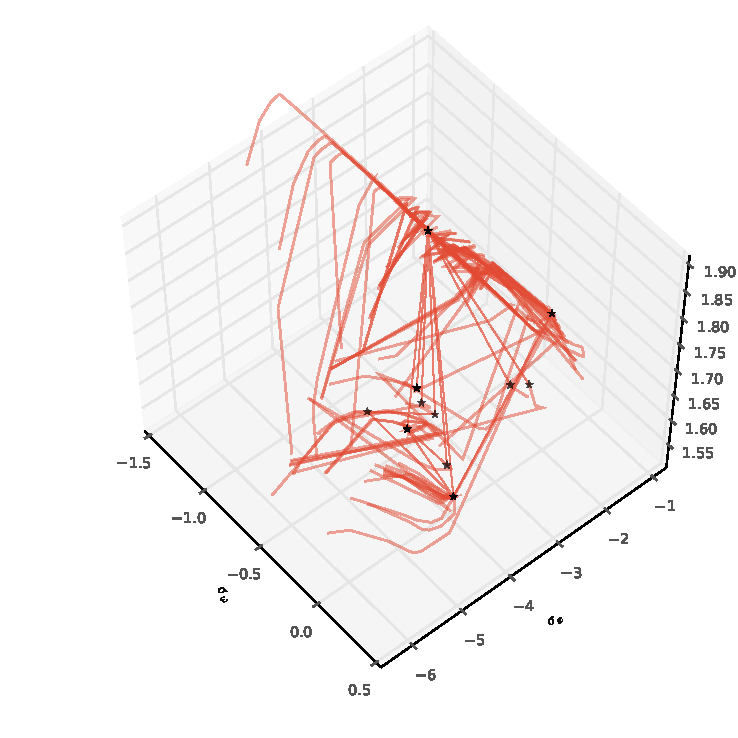
\includegraphics{img/harmonic_3D1}%
    \end{subfigure}
    \vspace*{-0.3cm}%
    \caption{Illustrations of the converge of the log-likelihood as a function of
    the logarithms of both $\sigma_\omega$ and $\sigma_x$ for EM (top) and
    BFGS (bottom). There are $100$ independent optimization runs per method with differing initial
    estimates, so that equal initial estimates were used between the methods. The end points
    of the runs are marked with black stars.}\label{fig:harmonic_3D}
 \end{figure}

 \begin{table}[htbp]
	\caption{Estimated final parameter and log-likelihood values in Section~\ref{sec:harmonic}.
	The value in parentheses is the amount of independent optimization runs averaged over. 
	The $\pm$ columns are the standard errors of the estimates in the preceding columns.
	BFGS($69$) is included, since some runs in BFGS($100$) converge to minor 
	local maximums of $\ell$.}
	\label{table:harmonic_results}
	\centering
	\sisetup{
		table-auto-round,
		table-format = 1.3
	}
	\footnotesize
	\begin{tabular}{rS[table-format=1.3,table-omit-exponent]S[table-format=1.1e2]S[table-format=1.3,table-omit-exponent]S[table-format=1.1e2]S[table-format=1.3,table-omit-exponent,fixed-exponent=4]S[table-format=1.1e2]}
\toprule
&\multicolumn{1}{c}{{\bfseries $\sigma_\omega$}}&\multicolumn{1}{c}{{\bfseries $\pm$}}&\multicolumn{1}{c}{{\bfseries $\sigma_x$}}&\multicolumn{1}{c}{{\bfseries $\pm$}}&\multicolumn{1}{c}{{\bfseries $\ell/\num{e4}$}}&\multicolumn{1}{c}{{\bfseries $\pm$}}\\\otoprule
EM($100$)&8.67068e-01&1.37391e-02&3.75632e-02&7.67759e-06&1.90778e+04&9.00616e-02\\
BFGS($100$)&8.44341e-01&3.90716e-02&3.22780e-02&2.80418e-03&1.86376e+04&6.71561e+01\\
BFGS($69$)&6.22636e-01&4.17172e-06&3.73572e-02&1.64853e-08&1.90790e+04&2.41266e-08\\
\bottomrule\end{tabular}

\end{table} 

 
 

